% ============================================================================
% reSTITCHing: Refining STITCH
% Journal-extension draft (REFERENCE DRAFT v7)
% ----------------------------------------------------------------------------
% Self-contained: compiles on its own in Overleaf.
% No em-dashes anywhere (commas / colons / parentheses used instead).
%
% v6 corrected the Set 3 framing from "escalation wins outright on strong
% models" (a pooled bump the replicate-level trace showed to be sampling
% noise, no semantic_fired win underneath) to the honest and structurally
% unattackable claim: on large models escalation does no harm, matches
% baseline within noise, and strengthens its cost advantage.
%
% v7 adds Section 9 (Phase 3: a real-MPSoC case study, 990 runs, interpreter
% upgrade v3), wires it into the abstract, roadmap, conclusion and directions,
% and applies wording-only corrections found when the draft was re-checked
% against the raw logs: the Set 1 always-on deficit is stated at the strength
% of its evidence, Set 1 timeout cells are named, the Set 3 flip sentence is
% arithmetically exact, iteration caps are disclosed, the Twin comparators are
% stated one by one, and the five unresolved citations are defined.
% No number in Sections 1 to 8 was changed.
%
% Figures live in figures/ next to this file (\graphicspath below); upload the
% folder with the .tex to Overleaf. Each is a copy; regenerate from its source:
%   set1_cost_passrate.png          <- phase2/set1_analysis/fig1_cost_vs_passrate.png
%   set1_tier_split.png             <- phase2/set1_analysis/fig2_tier_split.png
%   twin_named_comparisons.png      <- phase2/twin_analysis_SET2/fig1_named_comparisons.png
%   fig_capability_ladder_full.png  <- phase2/set3_analysis/fig_capability_ladder_full.png
%   fig_harmful_regime_ladder.png   <- phase2/set3_analysis/fig_harmful_regime_ladder.png
%   fig_p3_*.png (3 used here)      <- phase3/evidence/phase3_run/figures/
%                                      (python phase3/runner/analyze_phase3.py)
% Section 9 is the short form of PHASE3_MPSOC.tex (same folder), which carries
% every Phase 3 table.
% ============================================================================

\documentclass[11pt]{article}

\usepackage[margin=1in]{geometry}
\usepackage{booktabs}
\usepackage{tabularx}
\usepackage{graphicx}
\usepackage{xcolor}
\usepackage{enumitem}
\usepackage{amsmath}
\usepackage{hyperref}
\hypersetup{colorlinks=true, linkcolor=blue!50!black, urlcolor=blue!50!black}
\graphicspath{{figures/}}

\title{\textbf{reSTITCHing: Refining STITCH}\\[4pt]
\large\textnormal{From Single-Run Illustrations to $N{=}3$ Evidence,
Cost-Controlled Semantic Escalation, and a Real-MPSoC Case Study}}
\author{Karthikeya Patana \and Yashwant Rajesh \and Aathira Sunil \and Durga Saranyu \and Sri Parameswaran \and Kamesh Chandrasekar \and Paresh Saxena \and Soumya Joshi}
\date{}

\begin{document}
\maketitle

% ============================================================================
% ABSTRACT
% ============================================================================
\begin{abstract}
The conference version of STITCH characterised its deterministic semantic
interpreter through four outcome regimes (enabling, protective, harmful, and
irrelevant), each demonstrated by a single module and model pair evaluated
once. That evidence was illustrative, and the paper said so. This extension
replaces single-run illustration with $N{=}3$ replication on an external
benchmark (RTLLM~v2.1, $42$ modules) across a six-model capability ladder
spanning $4$B to $32$B parameters, and reports what survives it. Two
interpreter illustrations replicate cleanly and anchor the mechanism. A
mechanistic input/output reachability asymmetry explains \emph{which} defect
classes the interpreter can act on, and lets us predict where a
tool-augmented repair loop can help before any experiment is run. A
conditional-escalation architecture delivers the interpreter's benefit at
$35$ to $45\%$ lower tool-invocation cost on the in-house benchmark and at
tier-specific rates up to $75\%$ at RTLLM scale. A central finding is
directional: firing a repair interpreter on \emph{every} iteration, the
conference design, sits about four points below baseline on the recoverable
band for small models ($4$B to $8$B), a deficit consistent in direction but
within sampling noise at $N{=}3$, while conditional escalation matches
baseline with a structural worst-case guarantee. On the larger models tested
the deficit is largely absent at the group level, and escalation matches
baseline within sampling noise while strengthening its tool-cost advantage.
Escalation is therefore the capability-safe choice across the whole ladder: it
removes the deficit on weak models, and it costs strong models nothing where
the intervention is not needed. A controlled fine-tuning twin comparison
(RTLCoder-Deepseek-v1.1 versus its un-fine-tuned base) shows no net
fine-tuning advantage at confirmatory scale, a negative result on an external
benchmark, though the fine-tuned model does hold a clear edge on
signal-processing modules. We harden the evaluation harness against three
silent harness defects (working directory, code-fence extraction, and pass
detection) that had been quietly perturbing measurements, replacing ad-hoc
string checks with a structural benchmark-aware interface, and report the
defects as a methodological caution for the subfield. Finally, having
established where the interpreter acts, we asked whether STITCH is useful on
real hardware, and found that it catches the defects a simulation-only loop
signs off. On an independently developed RISC-V MPSoC with a mesh
network-on-chip ($990$ runs, six models from $3$B to $14$B), a
simulation-only repair loop signs off $62\%$ of its runs with synthesis defects
intact, and STITCH brings that to $1\%$; interpreting the lint and synthesis
output beats showing it raw by $14.6$ points (cell-level $95\%$ CI $+3.5$ to
$+26.3$) with about $23\%$ fewer model calls and tokens; escalation reaches the
highest clean pass rate ($80\%$); and the repaired leaf modules restore
top-level synthesis of $4$- and $9$-router meshes, which simulation-only
repair never achieves. An additive, regression-gated interpreter upgrade
driven by those designs shows how STITCH's vocabulary can keep growing. The
contribution is not that STITCH
works in more places, but that we now know \emph{when} it works, \emph{how
much} it helps, \emph{at what cost}, and \emph{for which models}, on
replicated, tier-decomposed evidence rather than single-draw pooled averages.
\end{abstract}

% ============================================================================
% SECTION 1
% ============================================================================
\section{Why This Extension Exists: N=1 Is Not Enough}
\label{sec:why}

The conference paper's table of interpreter outcomes was built on
\emph{single runs}: one module, one model, one draw per condition. Its own
Limitations section is explicit that the reported percentages are point
estimates rather than measured effects. For a repair mechanism evaluated on a
stochastic generator, that gap matters more than it first appears. A model at
low temperature with no fixed seed can pass one draw and fail the next from
sampling alone, so a single-run cell that shows the interpreter ``winning''
cannot, on its own, distinguish a real mechanism from sampling variance.

Replication mostly confirms the conference results, but the cases it does not
confirm are exactly the ones that would have become false claims at $N{=}1$.
This extension re-runs the mechanism under replication and reorganises the
evidence around a single discipline: no interpreter claim is made without
$N{\geq}3$ replication and a \texttt{semantic\_fired} check reported in the
same cell it explains. We hold this discipline even when it retires a result
we would have liked to keep, including, as Section~\ref{sec:stitch-rtllm}
records, a pooled improvement on large models that the replicate-level trace
shows to be sampling noise rather than a fired mechanism. Section~\ref{sec:worked}
presents the cases that survive this bar. Section~\ref{sec:retire} presents
what replication retired, because the retirements define the mechanism's scope
as sharply as the successes define its power. Section~\ref{sec:escalate}
introduces the cost-controlled escalation architecture. Section~\ref{sec:harness}
reports the harness corrections as a methodological caution.
Section~\ref{sec:fullstudy} describes the full-scale RTLLM study.
Section~\ref{sec:twin} presents the confirmatory fine-tuning twin comparison.
Section~\ref{sec:stitch-rtllm}, the core new contribution, is the
tier-decomposed and capability-conditioned evidence for when STITCH's
escalation architecture acts, when it correctly stays out, and what it can and
cannot claim on each part of the capability ladder.
Section~\ref{sec:mpsoc} then asks whether STITCH is useful on a real
multiprocessor design, and how the interpreter can be kept robust as it meets
new code and new tool versions.

% ============================================================================
% SECTION 2
% ============================================================================
\section{Where STITCH Works: Replicated Cases}
\label{sec:worked}

We report cases where STITCH's mechanism produces a genuine, replicated
benefit. Two are the interpreter proper on proven illustrations, and one is a
mechanistic reachability result that generalises them. Every case here clears
the $N{=}3$ bar and, where the interpreter is involved, a
\texttt{semantic\_fired} check.

\subsection{Two Proven Interpreter Illustrations}
\label{sec:worked-illus}

The gated-input \texttt{UNUSEDSIGNAL} mechanism, the conference paper's
cleanest illustration, replicates $3/3$ on two modules and two models
(Table~\ref{tab:proven}). In \texttt{decoder\_3to8} and \texttt{mux4\_oe} the
model omits a declared gating port on iteration one, Verilator fires
\texttt{UNUSEDSIGNAL}, and the interpreter's targeted directive resolves the
module in two iterations, against a six-iteration failure for both controls on
gemma3:4b (the llama3.1 rows pass under the controls as well, in two to four
iterations). In every cell the \texttt{raw\_adv} control tracks
\texttt{baseline} exactly, isolating the effect to \emph{interpretation}, not
tool presence.

\begin{table}[htbp]
\centering
\caption{Two proven illustrations, $N{=}3$ at $T{=}0.1$.
\texttt{raw\_adv} matches \texttt{baseline} in every cell, isolating the
effect to interpretation.}
\label{tab:proven}
\small
\begin{tabularx}{\linewidth}{@{} l l X X X @{}}
\toprule
\textbf{Module} & \textbf{Model} & \textbf{baseline} & \textbf{raw\_adv} & \textbf{sem\_adv} \\
\midrule
decoder\_3to8 & gemma3:4b & FAIL\,|\,6 & FAIL\,|\,6 & \textbf{PASS\,|\,2} \\
decoder\_3to8 & llama3.1  & PASS\,|\,2 & PASS\,|\,2 & PASS\,|\,2 \\
mux4\_oe      & gemma3:4b & FAIL\,|\,6 & FAIL\,|\,6 & \textbf{PASS\,|\,2} \\
mux4\_oe      & llama3.1  & PASS\,|\,4 & PASS\,|\,4 & PASS\,|\,2 \\
\bottomrule
\end{tabularx}
\end{table}

On the enabling cells the interpreter also cuts token cost sharply, roughly
$5$ to $7\times$ against both controls, because it converts a six-iteration
failure into a two-iteration pass. These two illustrations are deliberately
the same mechanism (a gating input, \texttt{enable} or \texttt{oe}, that the
model declares but never reads) on two different toy modules. That similarity
is not an oversight: several other candidate modules were built to elicit the
same defect and discarded because they failed to isolate it, either because
the specification accidentally handed the model the answer, or because the
resulting defect was a missing default that the system prompt already forces
the model to supply. The two survivors are the cases where the gated-input
defect is produced cleanly and nothing else is confounded.

These are small modules, and a fair objection is that decoders and gated
multiplexers are primitive. The response is that primitives compose. A
forgotten output-enable on a multiplexer that is instantiated two hundred
times in a larger design is two hundred latent defects, and a unit-level
repair that reliably fixes the primitive is what keeps the system-level
design correct. The interpreter's value is not that it repairs toy modules,
but that it repairs a defect \emph{class} that recurs at every level of a
hierarchy.

\subsection{The Input/Output Reachability Asymmetry}
\label{sec:worked-asym}

A mechanistic result explains \emph{which} defect classes the interpreter can
reach, and it is the section most likely to transfer to repair mechanisms
beyond STITCH. A forgotten gating \emph{input} reliably produces the target
defect and reaches the interpreter. A forgotten \emph{output} does not,
because the model assigns declared outputs unprompted on iteration one
(Table~\ref{tab:asym}).

\begin{table}[htbp]
\centering
\caption{Forgotten inputs are reachable; forgotten outputs are not.
\texttt{sf} = \texttt{semantic\_fired}. The interpreter fires only where the
model actually produces the target defect. These are hand-built diagnostic
illustrations on gemma3:4b, not RTLLM data.}
\label{tab:asym}
\small
\begin{tabularx}{\linewidth}{@{} l l X c @{}}
\toprule
\textbf{Target class} & \textbf{Module} & \textbf{Iteration-1 behaviour} & \textbf{sf} \\
\midrule
Forgotten \emph{input}  & decoder\_3to8 & port declared, never read & 1 \\
Forgotten \emph{input}  & mux4\_oe      & \texttt{oe} never referenced & 1 \\
Forgotten \emph{output} & adder\_with\_overflow & output assigned unprompted & 0 \\
Forgotten \emph{output} & fsm\_next\_state\_error & output assigned on all paths & 0 \\
\bottomrule
\end{tabularx}
\end{table}

The explanation is a completeness asymmetry in autoregressive generation.
Assigning a declared output is a \emph{local} obligation: if the model
declares an output and never drives it, the code reads as visibly unfinished,
and the model tends to close that gap on its own. Consulting a declared input
is a \emph{non-local} obligation: a module that never reads a declared input
still compiles and reads as complete, so the omission is only visible by
reasoning about the whole module's intended behaviour, and the model does
sometimes leave it out.

This directly explains why \texttt{semantic\_fired} is $0$ on the output rows.
The interpreter fires only when Verilator emits \texttt{UNUSEDSIGNAL}, which
occurs when a declared signal is never read. A forgotten output does not
produce that diagnostic, and in practice the defect does not occur at all
because the model assigns the output unprompted. So $\texttt{sf}{=}0$ on the
output cases does not mean the interpreter failed; it means the target defect
never occurred, so there was correctly nothing for the interpreter to fire on,
and nothing for the underlying tools to flag either. The two classes are not
symmetric: one needs the interpreter, and the other is handled by the
generator itself before any tool is consulted.

The practical consequence is a scope claim sharper than the conference paper
could make. Reachability is a joint property of the tool and the generator's
failure distribution, and it must be measured per class rather than assumed.
\texttt{UNUSEDSIGNAL} on a gating input is not an arbitrary choice among
handled codes; it is the class where tool visibility and real model failure
are \emph{known} to overlap. A repair-mechanism designer can use this
reasoning to predict, before running any experiment, which defect classes a
given tool-plus-generator pairing can and cannot address.
Section~\ref{sec:stitch-rtllm} is consistent with this asymmetry structuring
the RTLLM-scale result: the floor-tier modules, where nothing helps, are
consistent with defects that sit outside the tool's visibility, a prediction
that the floor corpus lets us test (Section~\ref{sec:conclusion}).

% ============================================================================
% SECTION 3
% ============================================================================
\section{What Replication Retired, and Why It Matters}
\label{sec:retire}

Three larger-module candidates were built to test whether the proven mechanism
scales, and none survived. Two failed $N{=}3$ replication, and the third,
\texttt{alu\_with\_enable}, was retired as too easy after redesign. The
failures define the mechanism's boundary and are reported at equal weight with
the successes.

\textbf{Resampling variance can masquerade as a win.}
\texttt{datapath\_mux\_alu}/llama3.1 passed \texttt{sem\_adv} in $2$ of $3$
samples with \texttt{semantic\_fired}${=}0$ in all three: the interpreter
never fired. As a single-run cell this reads as a clean win; it is sampling
variance, and $N{=}3$ is what exposes it. The same failure mode reappears at
scale in Section~\ref{sec:stitch-rtllm}, where a pooled large-model
improvement dissolves under a replicate-level trace into draw-to-draw variance
with no fired mechanism underneath.

\textbf{A correct directive does not guarantee recovery.}
\texttt{instr\_decode\_unit}/gemma3:4b fired \texttt{UNUSEDSIGNAL} correctly
and still failed, regressing into an unrelated degenerate syntax loop the
interpreter has no vocabulary to reach. Reaching a defect and repairing it
are different things.

% ============================================================================
% SECTION 4
% ============================================================================
\section{Cost-Controlled Semantic Escalation}
\label{sec:escalate}

The conference paper's own harmful and protective regimes point to one
structural weakness in firing the interpreter on every iteration: it
intervenes when intervention is not needed, and occasionally derails a run
that was already converging. The escalation architecture fires the
interpreter only once a run is demonstrably stuck. We evaluate three
interpreter policies against two controls. The controls are \texttt{baseline}
(model plus simulator only) and \texttt{raw\_adv} (the Verilator and Yosys
tool layer added but its output fed to the model uninterpreted). The three
interpreter policies are:

\begin{itemize}[leftmargin=1.2em, itemsep=0.15em]
\item \textbf{\texttt{sem\_adv}} (always-on) fires the interpreter on every
iteration. This is the conference paper's design.
\item \textbf{\texttt{sem\_escalate}} begins in the baseline state, tracks
consecutive failures carrying the same normalised error signature, and after
two identical-signature failures escalates permanently to the interpreter
path.
\item \textbf{\texttt{sem\_escalate\_restart}} adds a blank-slate rewrite if a
run stays stuck even after escalation.
\end{itemize}

The \texttt{raw\_adv} control matters because it separates two distinct
sources of help. The tool layer itself (compile, lint, and synthesis feedback
from Icarus Verilog~\cite{iverilog}, Verilator~\cite{verilator} and
Yosys~\cite{yosys}, in the manner of AutoChip~\cite{autochip}) can rescue a
run without any semantic interpretation, and the interpreter's translation
layer sits on top of that. Keeping the two separate lets us attribute each
effect correctly rather than crediting the interpreter for what raw tool
feedback achieved.

The escalation design carries a structural guarantee that always-on
interpretation cannot: because escalation begins as baseline and deviates only
after baseline has already failed twice on the same signature, on any problem
baseline solves, escalation behaves identically to baseline. Its worst case is
therefore bounded below by baseline, up to the noise of the two probe
iterations (and up to the iteration-cap difference disclosed in
Section~\ref{sec:stitch-rtllm-scope}). Always-on \texttt{sem\_adv} has no such
floor, and Section~\ref{sec:stitch-rtllm} shows it sitting below baseline on
small models, a consistent but not significant deficit. This guarantee is
structural, not statistical: it follows from the control flow of the policy
rather than from any measured delta, so it needs no confidence interval to
defend. The entire value proposition of escalation rests on it: capture the
interpreter's benefit where the interpreter helps, while structurally refusing
to pay the interpreter's cost, or risk its deficit, where it does not.

\subsection{The Cost Result on the In-House Benchmark}
\label{sec:escalate-cost}

The defensible headline is efficiency (Table~\ref{tab:cost}). Escalation
invokes the heavyweight tools roughly $35$ to $45\%$ less often than
always-on \texttt{sem\_adv} and \texttt{raw\_adv}, while matching or exceeding
their pass rate. The two cost axes diverge: escalation reduces \emph{tool
invocations} but can \emph{increase} tokens on cells where it escalates and
then runs extra iterations. The efficiency claim is scoped to the
tool-invocation axis, and both axes are reported.

\begin{table}[htbp]
\centering
\caption{Cost per run, all $255$ Phase~1 runs. Efficiency claim scoped to the
heavyweight-tool axis; token cost reported and moves the other way.}
\label{tab:cost}
\small
\begin{tabularx}{\linewidth}{@{} X r r @{}}
\toprule
\textbf{Condition} & \textbf{mean tokens/run} & \textbf{Verilator+Yosys calls/run} \\
\midrule
baseline                & 4891 & 0.00 \\
raw\_adv                & 5354 & 2.61 \\
sem\_adv                & 4883 & 2.37 \\
\textbf{sem\_escalate}  & 5151 & \textbf{1.53} \\
\textbf{sem\_esc\_restart} & 4719 & \textbf{1.37} \\
\bottomrule
\end{tabularx}
\end{table}

\subsection{Replication Collapse in the Benchmark Premise}
\label{sec:escalate-collapse}

The Phase~1 benchmark also produced a methodological result. The run set was
derived from historical $N{=}1$ labels, and re-measured at $N{=}3$, $4$ of $5$
``real-test'' and $2$ of $3$ ``enabling'' cells do not reproduce the baseline
behaviour their category was defined by. This is concrete evidence that
single-run RTL-repair benchmarks can encode sampling noise as apparent
structure. The regression gate nonetheless holds: both proven illustrations
pass $4/4$ on strict pass/fail under the new conditions.

% ============================================================================
% SECTION 5 (compressed)
% ============================================================================
\section{Harness Hardening: A Methodological Caution}
\label{sec:harness}

Across this work we found and fixed three silent defects in the shared runner,
each verified before and after against golden references. We report them
briefly because the pattern, not any single bug, is the point.

\textbf{Defect A (simulator working directory).} The simulation invocation set
no working directory, so any testbench doing relative-path file I/O
(\texttt{\$readmemh}) could never resolve its data file, regardless of whether
the generated logic was correct. Disqualifying for every file-I/O design;
confirmed not to affect the conference benchmark.

\textbf{Defect B (unclosed code-fence extraction).} An unclosed
\texttt{```verilog} fence left the opening marker attached, corrupting
otherwise-compilable code. An audit found $58$ of $659$ generated files
($8.8\%$) affected.

\textbf{Defect C (pass-string mismatch).} The harness checked for the
case-sensitive substring \texttt{"PASS"} or \texttt{"ALL TESTS PASSED"}, but
RTLLM's testbenches emit \texttt{"Your Design Passed"}, which contains
neither. A full re-scan of $64$ completed runs found $20$ ($31\%$) silently
misclassified as failures, and worse, corrupted trajectories: a cell that
actually passed on iteration one was told the simulation failed and spent its
remaining iterations ``fixing'' already-correct code under a false signal.

All three are the same underlying fragility: a hardcoded assumption about a
benchmark's output format, buried in shared code, that silently produces
plausible-looking wrong numbers. This is a caution for the subfield, because a
$31\%$ silent misclassification rate is large enough to invert a published
comparison. As a direct consequence, the confirmatory harness routes every
pass/fail decision through a single \texttt{detect\_outcome($\cdot$,
benchmark)} function backed by a per-benchmark registry, with the benchmark
identifier a required argument at every call site and no default fallback: a
new benchmark must register its conventions in one place, and forgetting to do
so raises an error at import rather than a silent misclassification months
later. All confirmatory results in Sections~\ref{sec:twin}
and~\ref{sec:stitch-rtllm} use this hardened detector, regression-verified
against $64$ manually-adjudicated cells before any full run was launched.

% ============================================================================
% SECTION 6
% ============================================================================
\section{The Full Study: RTLLM at $N{=}3$ Confirmatory Scale}
\label{sec:fullstudy}

To test generalisation beyond the in-house suite we migrated to
RTLLM~v2.1~\cite{lu2024rtllm}, an external $50$-design benchmark. A batch
compatibility screen found $44$ of $50$ designs compatible with the Icarus
flow; the $6$ exclusions each have a distinct, documented cause, one of which
is a defect in RTLLM's own golden reference. Two further designs
(\texttt{edge\_detect}, \texttt{square\_wave}) were excluded after their
testbenches were found to pass with stuck-at-$0$ outputs, a weak-oracle defect
that would inflate pass rates for weak models. This leaves a $42$-module
confirmatory pool.

An initial five-module pilot completed only three modules before a thermal
stop, and showed no condition differentiation for an instructive reason: the
three modules span a ceiling (\texttt{counter\_12}), a floor (\texttt{accu}),
and a flat mid-point (\texttt{barrel\_shifter}), none in the band where
STITCH's effect is measurable. The pilot's real yield was a design constraint:
STITCH's effect is observable only on modules where baseline sometimes fails
but is recoverable, so results must be reported per-module against a
difficulty characterisation rather than as a single pooled figure.

\textbf{Module difficulty tiers} are defined empirically from the Twin run's
baseline pass rates (Section~\ref{sec:twin}), which cover the widest model
spread in this study. For each of the $42$ modules, the maximum pass rate
across the five Twin model-conditions defines the tier:
\begin{itemize}[leftmargin=1.2em, itemsep=0.1em]
\item \textbf{Ceiling} ($6$ modules, max pass rate $\geq 80\%$): easy for any
      capable model.
\item \textbf{Recoverable band} ($17$ modules, $20\%\leq\text{max}<80\%$):
      where any comparison could show discriminating power.
\item \textbf{Floor} ($19$ modules, max pass rate $<20\%$): hard for every
      model tested.
\end{itemize}
The STITCH-conditions analyses (Section~\ref{sec:stitch-rtllm}) inherit this
tier definition verbatim.

\textbf{Three confirmatory runs} on the pool follow, all using the hardened
harness of Section~\ref{sec:harness}. Section~\ref{sec:twin} presents Set~$2$,
a fine-tuning twin comparison: $5$ model-conditions $\times\;42$ modules
$\times\;N{=}3=630$ runs at $T{=}0.5$, baseline-only.
Section~\ref{sec:stitch-rtllm} presents Set~$1$, STITCH conditions on three
small models ($4$B to $8$B): $3$ models $\times\;4$ conditions $\times\;42$
modules $\times\;N{=}3=1{,}512$ runs at $T{=}0.1$, and Set~$3$, the same four
conditions on three larger models ($14$B to $32$B) restricted to the $17$
recoverable-band modules: $3$ models $\times\;4$ conditions $\times\;17$
modules $\times\;N{=}3=612$ runs at $T{=}0.1$. All three completed, with $0$,
$6$, and $2$ timeouts respectively (Section~\ref{sec:stitch-rtllm-scope}).

% ============================================================================
% SECTION 7
% ============================================================================
\section{Confirmatory Twin Comparison}
\label{sec:twin}

\subsection{Design}
\label{sec:twin-design}

RTLCoder-Deepseek-v1.1~\cite{rtlcoder,rtlcoder_hf} is fine-tuned on a curated
Verilog dataset from the same DeepSeek-coder-6.7b base weights~\cite{deepseekcoder}
already in our evaluation. This creates a natural experiment: identical base
weights, differing only in fine-tuning, so any performance gap isolates the
fine-tuning contribution. We add gemma3:4b~\cite{gemma3} and
llama3.1~\cite{llama3} as ladder context, and run RTLCoder under both its
native stub-completion prompt and the shared harness prompt, making prompt
format a measured variable rather than a confound. All models are served
locally through Ollama~\cite{ollama}.

The scope is $5$ model-conditions (RTLCoder native, RTLCoder shared,
deepseek-coder shared, gemma3:4b shared, llama3.1 shared) $\times\;42$ modules
$\times\;N{=}3 = 630$ pre-registered runs at $T{=}0.5$, matched across models
for comparability. Condition is fixed at \texttt{baseline}: this is a
\emph{model} comparison, not a STITCH evaluation. All $630$ runs completed
with zero errors.

\subsection{Fine-Tuning Twin Verdict: A Negative Result With a Real Exception}
\label{sec:twin-finetune}

Contrasting RTLCoder shared against deepseek-coder shared isolates the
fine-tuning effect at a matched prompt, and this is the section's most
notable finding. On the $17$ recoverable-band modules ($51$ runs per
model-condition) the totals are deepseek-coder shared $32/51$ ($62.7\%$),
RTLCoder native $29/51$ ($56.9\%$) and RTLCoder shared $21/51$ ($41.2\%$); we
state which comparison each sentence uses. At the shared prompt RTLCoder wins
$0$ modules, ties $13$, and loses $4$ (with $|\Delta|\leq 1$ as the tie
threshold, matching the $N{=}3$ noise floor used in
Section~\ref{sec:worked}), and the base model is ahead by eleven passes.
Confidence intervals overlap, so this is a lean rather than a knockout, but
the direction runs opposite the fine-tuning claim's own hypothesis: on this
external benchmark, at this scale and temperature, fine-tuning RTLCoder on its
curated Verilog dataset does not measurably improve its recoverable-band pass
rate over the un-fine-tuned base at the shared prompt, and on four modules it
is worse. Against deepseek-coder at RTLCoder's own native prompt the
comparison is a wash ($29/51$ versus $32/51$; $5$ wins, $6$ ties, $6$
losses).

The four shared-prompt losses are not random. Inspecting them individually,
they trace to a submodule-hierarchy mismatch, SystemVerilog dialect leakage, a
parameter-binding failure, and, on \texttt{fixed\_point\_substractor}, a
naming-memorisation artefact in which RTLCoder reproduces RTLLM's folder name
over the specification's own stated module name, identically under both
prompts. These are fine-tuning side effects, not sampling noise.

Fairness requires reporting where the fine-tuning genuinely helps, and it does,
on the recoverable band. Broken out by functional class, RTLCoder under its
native prompt clears every recoverable signal-processing module ($9/9$ runs,
three modules) and the recoverable Memory module ($3/3$ runs, \texttt{LFSR}),
and scores $2/6$ on the Control class (two modules) where the un-fine-tuned
deepseek-coder scores $0/6$. Across all $42$ modules the native prompt is
$9/15$ on signal-processing and $6/12$ on Memory. The net recoverable-band
verdict is therefore a lean against fine-tuning at the shared prompt and a
wash at the native prompt, because the fine-tuning trades ground it loses on
general arithmetic for ground it gains on signal-processing and control-heavy
designs. Negative results on external benchmarks are worth reporting precisely
because a positive claim exists in the literature; we report both the net
verdict and its functional-class structure rather than collapsing either into
a single headline.

\subsection{Prompt-Format Effect}
\label{sec:twin-prompt}

Contrasting RTLCoder native against RTLCoder shared isolates prompt format.
Across the $17$ recoverable-band modules, native wins $3$, shared wins $2$, and
$12$ tie under the $|\Delta|\leq 1$ rule, while in total native passes $29/51$
against shared's $21/51$. The module-level effect is inconsistent
(Figure~\ref{fig:twin-comparisons}); we report it as such and claim no
direction beyond noting the larger total.

\begin{figure}[htbp]
\centering
\includegraphics[width=\linewidth]{twin_named_comparisons.png}
\caption{The two named comparisons at RTLLM confirmatory scale.
(a) Fine-tuning twin: RTLCoder shared versus deepseek-coder shared, $17$
recoverable-band modules; the net verdict leans against fine-tuning at the
shared prompt ($0$ wins, $13$ ties, $4$ losses), and four modules
(\texttt{adder\_8bit}, \texttt{fixed\_point\_adder},
\texttt{fixed\_point\_substractor}, \texttt{RAM}) go against RTLCoder, while
\texttt{width\_8to16} ($1/3$ against $2/3$) is counted as a tie by the
threshold rule. (b) Prompt-format effect: native versus shared prompt for
RTLCoder, same $17$ modules; native wins $3$, shared wins $2$, most tie.}
\label{fig:twin-comparisons}
\end{figure}

\subsection{Verdict}
\label{sec:twin-verdict}

Two findings survive $N{=}3$ confirmatory scale. First, no net fine-tuning
advantage for RTLCoder on RTLLM ($0$ wins, $13$ ties, $4$ losses at the shared
prompt; a wash at the native prompt), with a per-class exception: a clear edge
on the recoverable signal-processing modules (and the single recoverable Memory
module), offset by losses on general arithmetic. Second, prompt format has a
modest, inconsistent effect ($3$-$2$-$12$). Twin's baseline pass rates also
serve a structural purpose: they define the difficulty tiers of
Section~\ref{sec:fullstudy} and anchor the capability ladder that the STITCH
analysis (Section~\ref{sec:stitch-rtllm}) operates over. Nothing in this
section runs STITCH; it is a controlled model comparison.

% ============================================================================
% SECTION 8
% ============================================================================
\section{STITCH at RTLLM Scale: When the Interpreter Acts and When It Stays Out}
\label{sec:stitch-rtllm}

The escalation architecture's claim is not that STITCH improves pass rate
everywhere. It is that STITCH's interpreter, gated by \texttt{sem\_escalate},
acts where the model produces reachable defects and stays out where it does
not. Two runs quantify this. Set~$1$ ($1{,}512$ runs, three small models,
$4$B to $8$B, all $42$ modules) establishes the tier structure and the
always-on deficit that escalation is designed to avoid. Set~$3$ ($612$ runs,
three larger models, $14$B to $32$B, the $17$ recoverable-band modules)
extends the analysis up the capability ladder and shows the deficit is a
small-model phenomenon at the group level.

\subsection{Scope}
\label{sec:stitch-rtllm-scope}

Set~$1$: three Ollama models ($3$ replicates each) across four conditions on
all $42$ modules, $T{=}0.1$. Of $1{,}512$ cells, $6$ ($0.4\%$) errored as
timeouts and are excluded and counted separately: five on \texttt{RAM} with
llama3.1 (\texttt{sem\_escalate} replicates $1$ to $3$,
\texttt{sem\_escalate\_restart} replicates $1$ and $3$), a recoverable-band
module, and one on \texttt{LIFObuffer} with deepseek-coder
(\texttt{sem\_escalate\_restart}, replicate $2$), a floor-tier module. This is
why Table~\ref{tab:tier-pass} shows denominators of $150$ and $151$ in place
of $153$ on the recoverable band, and $170$ in place of $171$ on the floor.
\texttt{RAM}/llama3.1 is $0/3$ under both baseline and \texttt{sem\_adv}, so
counting the missing runs as failures moves the recoverable-band rates to
$47/153$ ($30.7\%$) for \texttt{sem\_escalate} and $54/153$ ($35.3\%$) for
\texttt{sem\_escalate\_restart}, and no conclusion changes. Set~$3$:
\texttt{qwen2.5-coder:14b} and \texttt{qwen2.5-coder:32b}~\cite{qwen25coder},
and \texttt{gemma3:27b}~\cite{gemma3}, across the same four conditions on the
$17$ recoverable-band modules, $T{=}0.1$ (matched to Set~$1$ for direct
comparability). Of $612$ cells, $2$ ($0.3\%$) errored as transient timeouts
(both \texttt{qwen2.5-coder:32b}, one \texttt{comparator\_4bit} and one
\texttt{multi\_booth\_8bit}); excluded and counted. Both runs use the hardened
\texttt{detect\_outcome} registry (Section~\ref{sec:harness}). Intervals are
Wilson $95\%$ intervals~\cite{wilson1927} throughout.

\textbf{Iteration budget.} In Sets~$1$ and~$3$, \texttt{baseline} and
\texttt{sem\_adv} were capped at six iterations and the two escalation
policies at eight; the Twin baselines that define the tiers ran with a cap of
eight. The extra iterations rarely mattered: on the recoverable band, one
\texttt{sem\_escalate} pass and one \texttt{sem\_escalate\_restart} pass in
Set~$1$ arrived only in iterations seven or eight ($47/150$ becomes $46/150$
and $54/151$ becomes $53/151$ at a cap of six), and none in Set~$3$. At an
equal cap of six, \texttt{sem\_escalate\_restart} is $53/151$ ($35.1\%$)
against baseline's $54/153$ ($35.3\%$), so no conclusion changes. The Phase~3
experiment of Section~\ref{sec:mpsoc} uses one shared budget for every
condition.

\subsection{The Tier-Decomposed Pass-Rate Story (Set~1)}
\label{sec:stitch-rtllm-pass}

Pooled across all $42$ modules, the four conditions land within $1.6$
percentage points of each other ($28.8\%$, $27.2\%$, $27.7\%$, $28.8\%$ for
baseline, sem\_adv, sem\_escalate, sem\_escalate\_restart). That flatness is
not evidence of no effect; it is exactly what the pilot predicted, since
pooling ceilings and floors dilutes any recoverable-band signal. Split by tier
(Figure~\ref{fig:tier-split}, Table~\ref{tab:tier-pass}), the structure the
pool hides becomes visible.

\begin{figure}[htbp]
\centering
\includegraphics[width=\linewidth]{set1_tier_split.png}
\caption{Set~$1$ pass rate by STITCH condition, split by difficulty tier
inherited from the Twin run. Error bars are Wilson $95\%$ CIs. On the
recoverable band, \texttt{sem\_adv} sits below baseline (the intervals
overlap), and \texttt{sem\_escalate\_restart} matches baseline. On ceilings and
floors all conditions coincide.}
\label{fig:tier-split}
\end{figure}

\begin{table}[htbp]
\centering
\caption{Pass counts by tier and STITCH condition, Set~$1$
($3$ small models $\times$ $N{=}3$).}
\label{tab:tier-pass}
\small
\begin{tabularx}{\linewidth}{@{} l X c c c c @{}}
\toprule
\textbf{Tier} & \textbf{Modules} & \textbf{baseline} & \textbf{sem\_adv} & \textbf{sem\_esc} & \textbf{sem\_esc\_restart} \\
\midrule
Ceiling      & $6$  & $44/54$   & $44/54$   & $\mathbf{46/54}$   & $43/54$ \\
Recoverable  & $17$ & $54/153$  & $47/153$  & $47/150$           & $\mathbf{54/151}$ \\
Floor        & $19$ & $11/171$  & $12/171$  & $11/171$           & $11/170$ \\
\midrule
\textbf{Pooled} & $42$ & $109/378$ & $103/378$ & $104/375$ & $108/375$ \\
& & ($28.8\%$) & ($27.2\%$) & ($27.7\%$) & ($28.8\%$) \\
\bottomrule
\end{tabularx}
\end{table}

Three findings, in order of confidence. \textbf{(1) Always-on interpretation
sits below baseline on the recoverable band, in direction, but not
significantly.} \texttt{sem\_adv} is about four points below baseline
($30.7\%$ versus $35.3\%$; the Wilson intervals overlap heavily,
Figure~\ref{fig:tier-split}). At the level of the $51$ module-by-model cells it
is worse in $7$ (ten replicates in total), better in $3$ (three replicates) and
equal in $41$; the cell-bootstrap $95\%$ interval of the pooled difference is
$-10.5$ to $+0.7$ points, so the deficit is not distinguishable from zero at
$N{=}3$, and it is not uniform across models (\texttt{gemma3:4b} and
\texttt{llama3.1} drop, \texttt{deepseek-coder} is unchanged). It is the
direction the conference paper's harmful regime predicted from a single cell,
and it is consistent with the view that always-on intervention is not free,
but Set~$1$ has no \texttt{raw\_adv} condition, so it cannot separate an
effect of the interpreter's directives from an effect of the raw tool text
they accompany. We treat it as a directional observation, and the escalation
argument of Section~\ref{sec:escalate} does not depend on it.
\textbf{(2) Escalation matches baseline on the recoverable band.}
\texttt{sem\_escalate\_restart} reaches $54/151$ ($35.8\%$) against baseline's
$54/153$ ($35.3\%$), the worst-case-equals-baseline guarantee of
Section~\ref{sec:escalate} observed at scale. \textbf{(3) Ceilings and floors
behave as designed.} On ceilings all four conditions produce essentially the
same pass rate ($80$ to $85\%$); on floors all four produce $6$ to $7\%$,
consistent with the defects there sitting outside the interpreter's reachable
class (Section~\ref{sec:worked-asym}), a prediction we have not yet tested.

\subsection{The Tier-Decomposed Cost Story (Set~1)}
\label{sec:stitch-rtllm-cost}

The pass-rate story would be a null result if escalation cost the same as
\texttt{sem\_adv} everywhere. It does not (Table~\ref{tab:tier-cost}).

\begin{table}[htbp]
\centering
\caption{Mean heavyweight-tool invocations per run, Set~$1$, by tier.
\texttt{baseline} is structurally $0$. The reduction column is
\texttt{sem\_escalate} relative to \texttt{sem\_adv}.}
\label{tab:tier-cost}
\small
\begin{tabularx}{\linewidth}{@{} l X r r r @{}}
\toprule
\textbf{Tier} & \textbf{Modules} & \textbf{sem\_adv} & \textbf{sem\_esc} & \textbf{Reduction} \\
\midrule
Ceiling            & $6$  & $4.02$ & $1.00$ & $\mathbf{75.1\%}$ \\
Recoverable band   & $17$ & $6.74$ & $5.62$ & $16.6\%$ \\
Floor              & $19$ & $7.28$ & $6.54$ & $10.1\%$ \\
\midrule
\textbf{Pooled}    & $42$ & $6.60$ & $5.38$ & $18.5\%$ \\
\bottomrule
\end{tabularx}
\end{table}

\begin{figure}[htbp]
\centering
\includegraphics[width=0.95\linewidth]{set1_cost_passrate.png}
\caption{Set~$1$, $1{,}512$ runs. (a) Mean Verilator+Yosys invocations per
run: escalation cuts the heavyweight-tool axis against always-on
\texttt{sem\_adv}, pooled across all $42$ modules. (b) Pooled pass rate holds
within $1.6$ points across all four conditions, the regression check the cost
claim requires.}
\label{fig:set1-cost}
\end{figure}

The reduction follows a clean monotonic gradient by tier: $75.1\%$ on
ceilings, $16.6\%$ on the recoverable band, and $10.1\%$ on floors. On modules
where baseline succeeds, escalation's two-strike gate almost never fires (the
tool call rate drops from $4.02$ to $1.00$ per run), while pass rate holds. On
the recoverable band and floor, escalation does trigger, because runs do get
stuck. Escalation's cost discipline concentrates on the modules where tools
have the least to offer, not by explicit policy but as a byproduct of the
two-strike gate tracking recoverability. The pooled $18.5\%$ is smaller than
Phase~1's $35$ to $45\%$ because RTLLM's mix is dominated by ceilings and
floors; the tier-level gradient is what is stable. The token axis moves the
other way, as on the in-house benchmark: escalation spends more tokens per run
because escalated runs execute additional iterations. The efficiency claim is
scoped throughout to the heavyweight-tool axis.

\subsection{Up the Capability Ladder: The Deficit is a Small-Model Phenomenon (Set~3)}
\label{sec:stitch-rtllm-set3}

Set~$1$ shows escalation avoiding the always-on deficit on small models.
Set~$3$ asks what happens as capability rises, running the same four
conditions on three larger models ($14$B to $32$B) over the same $17$
recoverable-band modules at the same temperature. The finding is that the
deficit largely disappears at the group level: the mean \texttt{sem\_adv}
minus baseline delta rises from $-4.6$ points on the small models (Set~$1$) to
$-0.65$ points on the large models (Set~$3$, Figure~\ref{fig:harm-ladder}).
Always-on interpretation stops trailing baseline once the models are strong
enough to get stuck less often.

Pooled across the three larger models (Table~\ref{tab:set3-pooled}), all four
conditions land within about three points of each other, with the two
escalation policies nominally highest (\texttt{sem\_escalate} $58.8\%$,
\texttt{sem\_escalate\_restart} $58.3\%$) and \texttt{baseline} at $56.2\%$.
We do not claim this as a win. A replicate-level trace of the $153$
\texttt{sem\_escalate} runs shows why: $88$ passed without ever escalating
(the model succeeded in the first two iterations, tools never engaged), $65$
escalated, and of those only $2$ eventually passed, neither with the semantic
interpreter having fired (\texttt{semantic\_fired}${=}0$ throughout, both
rescued by raw Verilator and Yosys feedback after escalation, within the first
six iterations). Across all $153$ \texttt{sem\_escalate} runs, not a single
passing replicate had the interpreter fire (for
\texttt{sem\_escalate\_restart}, one of its $88$ passing runs had the
interpreter fire, and seven of \texttt{sem\_adv}'s $85$). The net pooled
improvement over baseline ($+4$ replicates, $90$ versus $86$ of $153$) comes
from six of the $51$ cells gaining seven replicates in total against three
cells losing one each, and every confidence interval crosses zero. This is the
same resampling-variance pattern Section~\ref{sec:retire} describes, now at
scale: independently drawn $N{=}3$ samples differ by exactly the amount
sampling noise predicts, and there is no fired mechanism underneath. The
honest reading is that on large models escalation does no harm and matches
baseline within noise, which is precisely what the structural guarantee of
Section~\ref{sec:escalate} promises and all it promises.

\begin{table}[htbp]
\centering
\caption{Set~$3$ pooled recoverable-band pass rate, three larger models
($14$B to $32$B) $\times$ $N{=}3$, $T{=}0.1$. All four conditions coincide
within noise; the escalation lead is not a fired-mechanism effect (see text).}
\label{tab:set3-pooled}
\small
\begin{tabularx}{\linewidth}{@{} X c c @{}}
\toprule
\textbf{Condition} & \textbf{Passes / n} & \textbf{Rate} \\
\midrule
baseline                     & 86/153 & $56.2\%$ \\
sem\_adv                     & 85/153 & $55.6\%$ \\
sem\_escalate                & 90/153 & $58.8\%$ \\
sem\_esc\_restart            & 88/151 & $58.3\%$ \\
\bottomrule
\end{tabularx}
\end{table}

The per-model picture (Table~\ref{tab:set3-permodel}) confirms the deficit is
model-specific rather than a smooth function of scale.
\texttt{gemma3:27b} reverses it, with \texttt{sem\_adv} $7.8$ points above its
baseline, while \texttt{qwen2.5-coder:32b}, the most capable model, still shows
a $-5.9$-point deficit comparable to a small model's. Reporting this
non-monotonicity is the honest counterpart to not claiming the pooled lead:
the effect that is real (per-model differences on some models) and the effect
that is not (a general escalation pass-rate win) are separated rather than
averaged into a single misleading number.

\begin{table}[htbp]
\centering
\caption{Set~$3$ per-model recoverable-band pass rate ($n{=}51$ per cell,
except \texttt{qwen2.5-coder:32b} sem\_esc\_restart $n{=}49$ after two
timeouts). The \texttt{sem\_adv} column shows the always-on deficit is
model-specific: present on \texttt{qwen2.5-coder:32b}, reversed on
\texttt{gemma3:27b}.}
\label{tab:set3-permodel}
\small
\begin{tabularx}{\linewidth}{@{} X c c c c @{}}
\toprule
\textbf{Model} & \textbf{baseline} & \textbf{sem\_adv} & \textbf{sem\_esc} & \textbf{sem\_esc\_restart} \\
\midrule
qwen2.5-coder:14b & $52.9\%$ & $49.0\%$ & $56.9\%$ & $58.8\%$ \\
gemma3:27b        & $37.3\%$ & $45.1\%$ & $37.3\%$ & $33.3\%$ \\
qwen2.5-coder:32b & $78.4\%$ & $72.6\%$ & $82.4\%$ & $83.7\%$ \\
\bottomrule
\end{tabularx}
\end{table}

\begin{figure}[htbp]
\centering
\includegraphics[width=\linewidth]{fig_harmful_regime_ladder.png}
\caption{Always-on interpretation's deficit (\texttt{sem\_adv} minus baseline,
percentage points on the recoverable band) against model capability, all six
models, $N{=}3$, $T{=}0.1$. Set~$1$ small models in red, Set~$3$ large models
in blue, ordered by baseline pass rate. The group mean deficit shrinks from
$-4.6$ (small) to $-0.65$ (large), but per-model the effect is not monotonic:
\texttt{gemma3:27b} reverses it while \texttt{qwen2.5-coder:32b} retains it.
Wilson $95\%$ CIs, all crossing zero on the large models.}
\label{fig:harm-ladder}
\end{figure}

The cost discipline, unlike the pass rate, does hold and strengthen at scale.
On the recoverable band, the \texttt{sem\_adv} to \texttt{sem\_escalate}
tool-invocation reduction is $27.6\%$ for the Set~$3$ models ($5.31$ to $3.85$
calls per run), against $16.6\%$ for the Set~$1$ models on the identical
module band. Capable models get stuck less often, so escalation triggers its
heavyweight path less often, and the cost advantage over always-on
interpretation widens. This is a real effect, not a noise artefact: it is a
per-run mechanical count of tool invocations, not a pass-rate delta.

The extended capability ladder (Figure~\ref{fig:capability-full}) places all
six models on a single axis spanning $4$B to $32$B, confirming that the range
is well covered and that the strong models sit where expected. Because Set~$3$
runs at $T{=}0.1$ and the Twin models at $T{=}0.5$, the comparison across the
two temperatures is ordinal (the ladder ordering) rather than a direct
rate match, and the figure marks this.

\begin{figure}[htbp]
\centering
\includegraphics[width=\linewidth]{fig_capability_ladder_full.png}
\caption{Full capability ladder, $4$B to $32$B, eight model-conditions on the
$17$ recoverable-band modules, \texttt{baseline}. Twin (Set~$2$, $T{=}0.5$) in
orange, Set~$3$ ($T{=}0.1$) in blue; the two colours are an ordinal comparison
only, since temperature differs. Wilson $95\%$ CIs, $n{=}51$ per bar.}
\label{fig:capability-full}
\end{figure}

\subsection{What This Establishes}
\label{sec:stitch-rtllm-summary}

Read together with Sections~\ref{sec:worked} and~\ref{sec:escalate}, the two
STITCH runs support five claims:
\begin{enumerate}[leftmargin=1.2em, itemsep=0.15em]
\item The proven-illustration mechanism (Section~\ref{sec:worked-illus})
generalises to a per-tier prediction: the interpreter helps where it can reach
a real defect and stays silent where it cannot.
\item Always-on interpretation shows a deficit of about four points on the
recoverable band of the three small models, consistent in direction (worse in
$7$ of $51$ cells, better in $3$) but within sampling noise at $N{=}3$
(cell-bootstrap $95\%$ CI $-10.5$ to $+0.7$ points), and not separable from
the effect of the raw tool text it accompanies, since Set~$1$ has no
\texttt{raw\_adv} condition. We report it as a directional finding, not an
isolated cause.
\item Escalation matches baseline on the recoverable band for the small
models, and on large models matches baseline within noise. The
worst-case-equals-baseline guarantee holds across the whole ladder, and it is
structural rather than statistical.
\item The deficit is a small-model phenomenon at the group level: it fades as
capability rises, though per-model it is not monotonic (\texttt{gemma3:27b}
reverses it, \texttt{qwen2.5-coder:32b} retains it). We do not claim a
large-model pass-rate win for escalation; the pooled lead is sampling noise
with no fired mechanism underneath.
\item The cost result is tier-shaped and strengthens with capability:
escalation cuts about three-quarters of heavyweight-tool calls on ceilings and
its recoverable-band reduction rises from $16.6\%$ on small models to $27.6\%$
on large ones. This is a mechanical per-run count, unaffected by the pass-rate
noise.
\end{enumerate}
None of this establishes STITCH as a universal pass-rate improvement; the
pooled numbers and the replicate-level trace make that explicit. It establishes
something narrower and more defensible: always-on interpretation, the
conference design, shows a consistent but not significant deficit on weak
models, and conditional escalation is the mechanism that captures the
interpreter's benefit where it fires while structurally guaranteeing a
baseline-level worst case and lower tool cost everywhere else. On weak models
that guarantee removes the deficit; on strong models it is a promise kept at no
cost. That is a sharper claim than a broad pass-rate win, and it rests on
$2{,}124$ replicated STITCH-condition runs (Sets~$1$ and~$3$).

RTLLM scores a module by its testbench alone, and on its recoverable band the
interpreter found something to say in only about a third of always-on runs
($52$ of $153$ in Set~$1$). STITCH's benefit scales with the structural share
of a failure, which is why RTLLM pass rates stay flat. RTLLM cannot measure
what STITCH was built for in the first place: defects that pass the testbench
and still break synthesis, and that multiply when a module is instantiated
across a real design. Section~\ref{sec:mpsoc} takes STITCH there.

% ============================================================================
% SECTION 9 (Phase 3): STITCH on a Real MPSoC
% Full write-up with every table: PHASE3_MPSOC.tex. Numbers: phase3/evidence/
% phase3_run/PHASE3_RESULTS.md (generated by phase3/runner/analyze_phase3.py).
% ============================================================================
\section{Is STITCH Useful on Real Hardware? An MPSoC Case Study}
\label{sec:mpsoc}

Sections~\ref{sec:worked} to~\ref{sec:stitch-rtllm} establish when STITCH acts
on single-module benchmarks, and Section~\ref{sec:worked-illus} rested on an
argument those benchmarks could not test: primitives compose, so a defect
repaired once in a leaf definition is repaired in every instance of it. Here
we test that argument on a design nobody wrote for this study, and ask the
practical question behind it: does STITCH catch the defects that decide
whether a real multiprocessor design can be signed off? The design's own logs first called for an interpreter upgrade;
$990$ repair runs then give five results.

\subsection{Substrate: a Real MPSoC That Already Contains the Target Defects}
\label{sec:mpsoc-substrate}

The design is an in-group MPSoC: a five-stage RV32 core, a network interface
(packetiser, depacketiser, and asynchronous FIFOs), and a virtual-channel
wormhole mesh router, available as a $2{\times}2$ mesh ($4$ routers) and a
$3{\times}3$ mesh ($9$ routers) that share $28$ of $33$ router leaf files. The
only changes made were compile-level ones required by the open-source flow
(redeclarations, nested comments, and Vivado-style implicit trailing ports,
reproduced with identical binding); no structural defect was touched.

The reference design already contains the defect classes STITCH targets.
Synthesis of the MPSoC top reports $63$ latch inferences across $12$ module
definitions and then aborts outright: a one-bit register cell tests
\texttt{clr | reset} inside an asynchronous-reset block, which Yosys cannot
map. These defects are \emph{simulation-silent}: every latch-bearing
multiplexer we examined behaves correctly on its intended inputs, and the
aborting register simulates correctly. A simulation-only repair loop has
nothing to react to. Because the top-level testbench is a weak oracle (it
executes two instructions and never exercises the network), all top-level
claims below are structural; functional claims rest on per-module,
specification-based testbenches.

\subsection{Defects Propagate With Instance Count; the Feedback Does Not}
\label{sec:mpsoc-propagation}

Both meshes inherit two defective register definitions ($32$ and $4$ latched
bits), each instantiated $20$ times per router (Table~\ref{tab:mpsoc-prop}).

\begin{table}[htbp]
\centering
\caption{Composition of two leaf-level defects in the real mesh routers.
Yosys prints one latch message per module \emph{definition}, so the feedback a
repair loop sees is identical at $N{=}4$ and $N{=}9$, while the physical damage
scales exactly with router count ($6{,}480/2{,}880 = 9/4$). Repairing the three
defective leaf definitions restores both meshes.}
\label{tab:mpsoc-prop}
\small
\begin{tabularx}{\linewidth}{@{} X c c @{}}
\toprule
 & \textbf{$2{\times}2$ mesh ($N{=}4$)} & \textbf{$3{\times}3$ mesh ($N{=}9$)} \\
\midrule
Yosys latch messages               & $2$ & $2$ \\
Latch cells ($36 \times 20 \times N$) & $2{,}880$ & $6{,}480$ \\
Top-level synthesis, as written    & aborts & aborts \\
Top-level synthesis, $3$ leaves repaired & pass, $0$ latch cells & pass, $0$ latch cells \\
\bottomrule
\end{tabularx}
\end{table}

Propagation is therefore linear and predictable from instance multiplicity,
and the leverage of a leaf repair grows with $N$. For the full MPSoC,
repairing eight leaf modules turns a synthesis abort into a pass; $122$ latch
cells remain, all in five modules outside the repair set, so the achievable
claim at the MPSoC top is restored synthesisability rather than a latch-free
design.

\subsection{Keeping the Interpreter Robust: an Additive Upgrade}
\label{sec:mpsoc-v3}

Running the production interpreter of Sections~\ref{sec:worked}
to~\ref{sec:stitch-rtllm} on the real MPSoC logs exposed gaps that synthetic
tests had not. On the unused \emph{clock} of the latching registers, the
generic gating template directs the model to write \texttt{if (clk)} inside a
combinational block, which builds a clock-gated latch; the async-reset abort
produces no directive at all, and a width truncation whose operand is an
expression is dropped silently. We therefore added an additive layer (v3) that
imports the production interpreter unchanged, reproduces its output
byte-for-byte wherever no new rule applies, and adds rules only where a real
log showed the production directive wrong or missing. Its most consequential
rule is cross-tool fusion: a Yosys latch in a level-sensitive block together
with a Verilator unused-clock warning is diagnosed as a missing clock edge
rather than as either warning alone. The same discipline that hardened the
harness (Section~\ref{sec:harness}) applied here: a live drift gate, which runs
the interpreter on fresh tool output before any GPU time is spent, caught a
latch-message format change between the development toolchain (Yosys~$0.33$)
and the cluster toolchain (Yosys~$0.69$) that would otherwise have silently
disabled the new rules.

\subsection{Experiment}
\label{sec:mpsoc-exp}

The repair set has $11$ tasks: the $8$ defective real MPSoC leaves and $3$
seeded RISC-V/NoC modules covering classes absent from the reference (ALU flag
latches, a multi-driven crossbar output, and flit-packing truncation). Six of
the eleven are simulation-silent: the defective input passes its testbench.
Each run starts from the defective input, which is evaluated before the first
model call, so every condition's feedback reaches the model from call one. A
pilot with hint-bearing specifications let an $8$B model fix every defect on
its first call under every condition, the same confound that retired
candidates in Section~\ref{sec:worked-illus}; the final specifications are
purely behavioural and the prompt is identical across conditions.
Conditions are \texttt{baseline} (simulation only, stopping at the first
simulation pass, as AutoChip~\cite{autochip}), \texttt{raw\_adv},
\texttt{sem\_adv} with the production interpreter (v2) and with the upgraded
interpreter of Section~\ref{sec:mpsoc-v3} (v3), and \texttt{sem\_esc\_restart}
with v3. All share one budget of six model calls and identically filtered raw
tool text, so the conditions differ only in what is fed back. Six models from
$3$B to $14$B (llama3.2:3b, gemma3:4b, deepseek-coder:6.7b, qwen2.5-coder:7b,
llama3.1:8b, qwen2.5-coder:14b), $N{=}3$, $T{=}0.1$, run on the institutional
GPU cluster~\cite{bitshpc}: $990$ runs, all completed (three transient
timeouts were re-run). The primary metric is \texttt{clean\_pass}: the
testbench passes \emph{and} Yosys synthesises the module with no latch and no
loop \emph{and} Verilator reports no hard structural warning. Because the
three replicates of a (model, task) cell are correlated, general claims quote
a cell-level bootstrap interval over the $66$ cells, which is about $1.7$ times
wider than the per-run Wilson interval.

\subsection{Results}
\label{sec:mpsoc-results}

\begin{table}[htbp]
\centering
\caption{Phase~3, $990$ runs ($198$ per condition). \texttt{func\_pass}: the
testbench passes. \texttt{clean\_pass}: it passes and the module is
structurally clean. A silent structural pass is \texttt{func\_pass} without
\texttt{clean\_pass}: signed off, still defective. Wilson $95\%$ CIs.}
\label{tab:mpsoc-cond}
\small
\begin{tabularx}{\linewidth}{@{} X c c c r @{}}
\toprule
\textbf{Condition} & \textbf{func\_pass} & \textbf{clean\_pass} & \textbf{silent structural pass} & \textbf{tokens/run} \\
\midrule
baseline              & $85\%$ & $23\%$ ($18$ to $30$) & $62\%$ & $1{,}425$ \\
raw\_adv              & $65\%$ & $59\%$ ($52$ to $66$) & $6\%$  & $4{,}396$ \\
sem\_adv (v2)         & $71\%$ & $68\%$ ($61$ to $74$) & $3\%$  & $3{,}831$ \\
sem\_adv (v3)         & $74\%$ & $74\%$ ($67$ to $79$) & $1\%$  & $3{,}377$ \\
sem\_esc\_restart (v3) & $85\%$ & $\mathbf{80\%}$ ($74$ to $85$) & $5\%$ & $3{,}798$ \\
\bottomrule
\end{tabularx}
\end{table}

\begin{figure}[htbp]
\centering
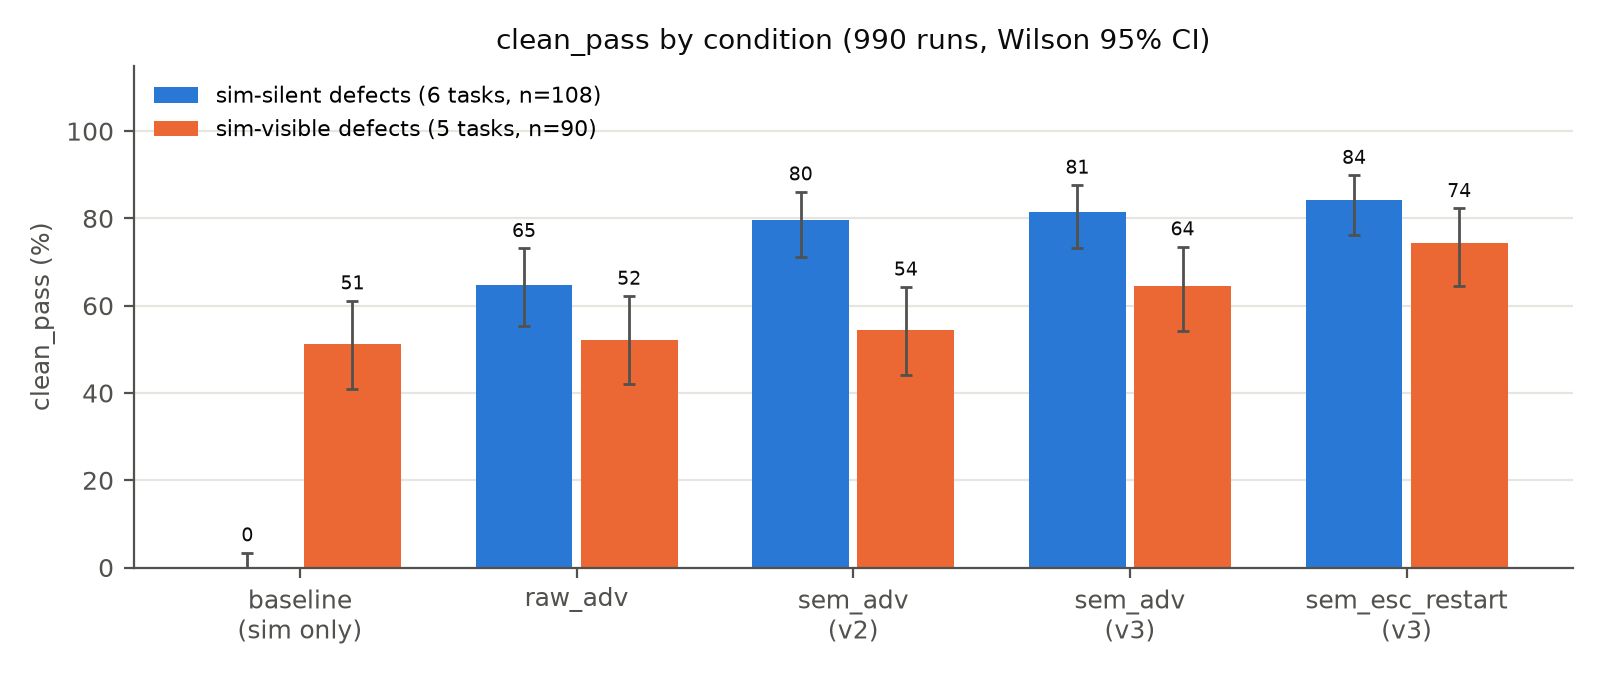
\includegraphics[width=\linewidth]{fig_p3_clean_by_condition.png}
\caption{\texttt{clean\_pass} by condition, split by whether the defect is
visible to simulation. On sim-silent defects, simulation-only repair scores
$0/108$ by construction; every tool condition recovers most of them.}
\label{fig:mpsoc-cond}
\end{figure}

\textbf{(1) STITCH catches what a simulation-only loop signs off.}
\texttt{baseline} reaches an $85\%$ simulation pass rate but only $23\%$
\texttt{clean\_pass}: $62\%$ of its runs are signed off with the defect
intact, and on the six sim-silent tasks it signs off all $108$, stopping
before any model call because the defective input already passes simulation
(Table~\ref{tab:mpsoc-cond}, Figure~\ref{fig:mpsoc-cond}). With the synthesis
and lint layer and the interpreter, silent structural passes fall to $1$ of
$198$ (v3), and on the latch-bearing tasks the runs that end latch-free with a
clean synthesis rise from $24\%$ to $88\%$. This is the structural blindness
that motivates a synthesis-aware loop, measured rather than argued.

\textbf{(2) Interpretation beats raw tool text, sooner and cheaper.} With the
same raw text and the same budget, \texttt{sem\_adv} (v3) reaches $146/198$
against \texttt{raw\_adv}'s $117/198$: $+14.6$ points, cell-level CI
$[+3.5, +26.3]$, with $43$ discordant pairs in its favour against $14$. The
production interpreter already beats raw text ($+9.1$, CI $[+1.0, +17.7]$), so
the value of interpretation does not depend on the upgrade. v3 gets there with
about $23\%$ fewer model calls and tokens per run, at $4{,}580$ against
$7{,}440$ tokens per clean pass, and $62\%$ of its runs are clean after the
first call, against $46\%$ for raw text and $17\%$ for simulation only
(Figure~\ref{fig:mpsoc-call}). The gain is largest where raw text is hardest to
use: $+24.2$ points on the $3$B model and $+27.3$ on qwen2.5-coder:7b, which
reaches $33/33$; the $14$B model is at $33/33$ with any tool feedback, so it
has nothing left to gain.

\begin{figure}[htbp]
\centering
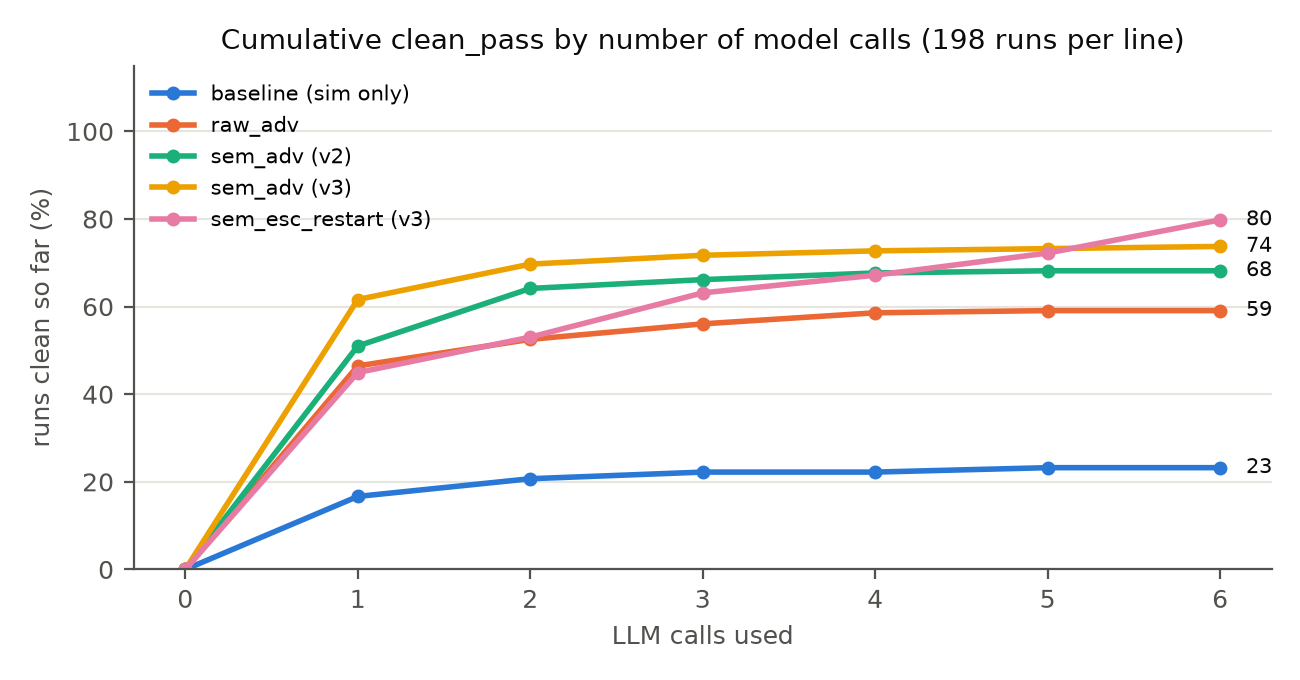
\includegraphics[width=0.85\linewidth]{fig_p3_clean_by_call.png}
\caption{Share of runs clean after each number of model calls ($198$ runs per
line). v3 front-loads its repairs; escalation, which begins as baseline, keeps
climbing to the highest final rate.}
\label{fig:mpsoc-call}
\end{figure}

\textbf{(3) Escalation reaches the highest clean rate with the fewest tool
rounds.} \texttt{sem\_esc\_restart} reaches $80\%$ \texttt{clean\_pass} and
keeps baseline's $85\%$ simulation pass rate, with $47.5\%$ fewer
tool-feedback rounds than always-on v3. On the sim-visible tasks, where
simulation-only repair does run the model, escalation beats it by $+23.3$
points ($67/90$ against $46/90$, cell-level CI $[+8.9, +37.8]$), and it
protects the smallest model: on those tasks llama3.2:3b is at $9/15$ with
simulation only, $1/15$ with raw text every round, and $8/15$ with
escalation. This is the Phase~3 counterpart of the capability-safety result of
Section~\ref{sec:stitch-rtllm}, now with one shared budget for every
condition.

\textbf{(4) Repaired leaves let the real designs synthesise.} Splicing each
(model, replicate) set of repaired leaves back into the real designs
(Table~\ref{tab:mpsoc-compose}, Figure~\ref{fig:mpsoc-compose}):
simulation-only repair never produces a synthesisable design ($0/18$ in all
three), because it never touches the sim-silent register that aborts
synthesis. v3 reaches $16/18$ in each design and escalation $18/18$ in both
meshes. Leaf-level \texttt{clean\_pass} was sufficient for composition in
every case: whenever all composed leaves were clean, the design reached the
bound of Table~\ref{tab:mpsoc-prop} ($32/32$, $32/32$, $27/27$), with no
composition-only failure.

\begin{table}[htbp]
\centering
\caption{Top-level synthesis pass of the real designs after splicing in each
condition's repaired leaves ($18$ model $\times$ replicate groups per cell).
Synthesis only; composed systems are not simulated.}
\label{tab:mpsoc-compose}
\small
\begin{tabularx}{\linewidth}{@{} X c c c c c @{}}
\toprule
\textbf{Design} & \textbf{baseline} & \textbf{raw\_adv} & \textbf{sem\_adv (v2)} & \textbf{sem\_adv (v3)} & \textbf{sem\_esc\_restart} \\
\midrule
$2{\times}2$ mesh & $0/18$ & $15/18$ & $13/18$ & $16/18$ & $\mathbf{18/18}$ \\
$3{\times}3$ mesh & $0/18$ & $15/18$ & $13/18$ & $16/18$ & $\mathbf{18/18}$ \\
MPSoC top         & $0/18$ & $13/18$ & $12/18$ & $\mathbf{16/18}$ & $15/18$ \\
\bottomrule
\end{tabularx}
\end{table}

\begin{figure}[htbp]
\centering
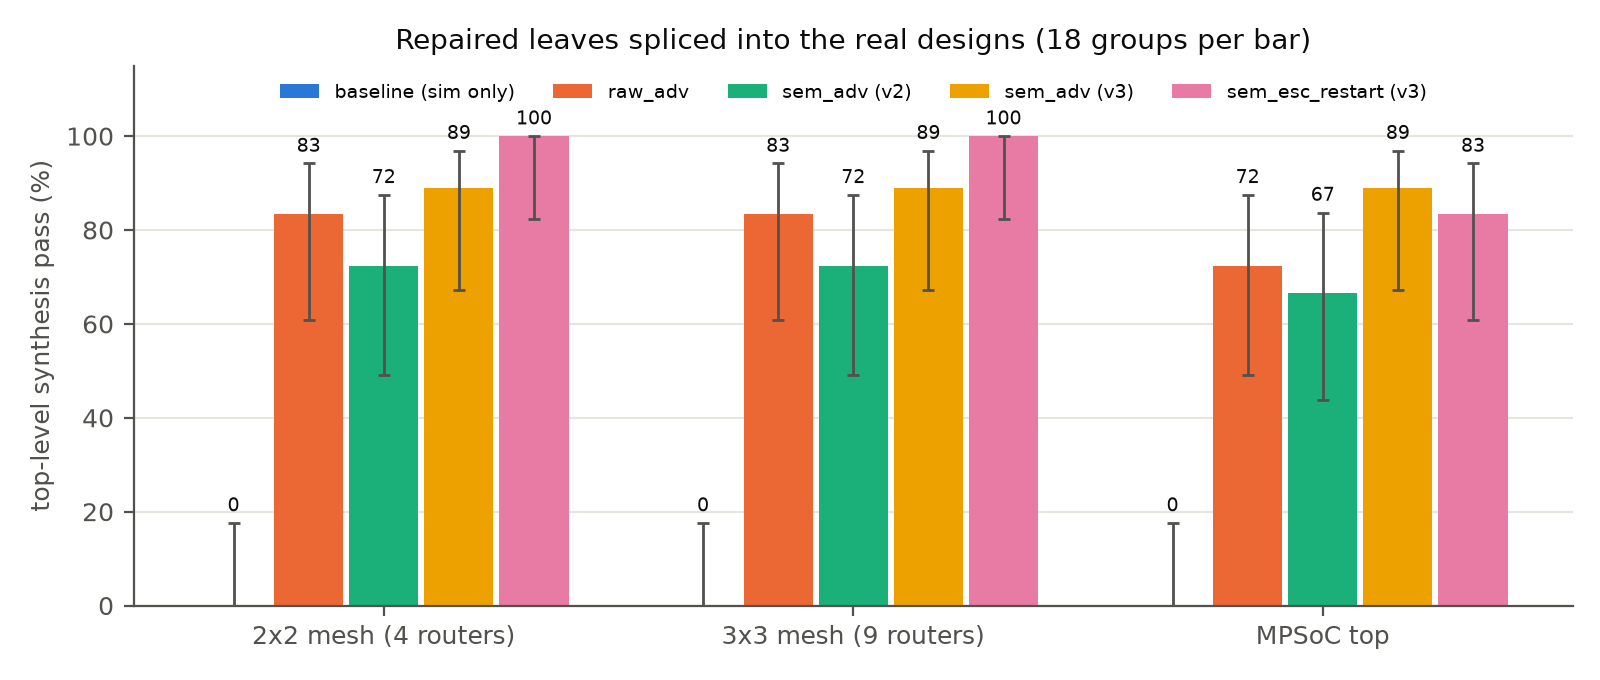
\includegraphics[width=\linewidth]{fig_p3_composition.png}
\caption{Top-level synthesis pass of the $2{\times}2$ mesh, $3{\times}3$ mesh
and MPSoC after splicing in repaired leaves, by condition, Wilson $95\%$ CIs.}
\label{fig:mpsoc-compose}
\end{figure}

\textbf{(5) The upgrade closes the vocabulary gaps.} The upgrade is first a coverage result. On the two tasks where the production
interpreter produced no directive on the defective input (the async-reset
register and the flit-packing truncation), v3 fires the intended class in
$18/18$ runs; on the two latching registers it replaces the clock-gating
directive with the missing-clock directive; and on the address selector it
drops a misleading ``gate the output on the instruction bus'' directive. On the
async-reset register, whose abort blocks synthesis of both meshes, the
interpreter-credited wins rise from $3/18$ to $15/18$. Across the four tasks
singled out before the runs, clean passes rise from $42/72$ to $50/72$
($+11.1$ points, cell-level CI $[-9.7, +31.9]$): a favourable direction that
the next runs, on held-out defects, are designed to confirm.

\subsection{What the Case Study Establishes}
\label{sec:mpsoc-summary}

On real multiprocessor RTL, the question STITCH answers is not whether a module
simulates but whether the design can be signed off. There, a simulation-only
loop is structurally blind, the synthesis and lint layer is what makes the
defects visible, and interpretation turns that visibility into repairs more
reliably, sooner and more cheaply than raw tool text. Leaf repairs compose:
fixing a handful of definitions restores synthesis of networks with $4$ and
$9$ routers. The case study also shows how the interpreter should evolve: new
real designs expose missing vocabulary, and additive, regression-gated
upgrades close those gaps without disturbing earlier results. Its scope is
equally clear, and sets the next runs: the v3 rules are in-sample until tested
on held-out defects; defects that exist only at composition (a one-bit
program-counter port driven with $32$ bits, a FIFO instantiated positionally
with a missing port) need integration-level feedback; and a control arm that
gives baseline escalation's generic sign-off message will separate being told
\emph{that} sign-off failed from being told \emph{what} failed.

% ============================================================================
% SECTION 10
% ============================================================================
\section{Conclusion and Directions}
\label{sec:conclusion}

The conference version of STITCH showed the interpreter could help, via four
single-run outcome regimes on hand-selected cells. This extension replaces
that evidence with $N{=}3$ replicated, tier-decomposed evidence across $42$
modules and a six-model $4$B-to-$32$B ladder on an external benchmark, and
answers four questions the conference paper deferred. \emph{When} does the
interpreter help: on the recoverable band, on small models, and only when the
model produces a defect from the reachable input class
(Section~\ref{sec:worked-asym}). \emph{How much}: firing the interpreter every
iteration leaves small models about four points below baseline on the
recoverable band (a consistent direction, within sampling noise at $N{=}3$),
and escalation matches baseline; on large models the deficit is largely absent
and escalation matches baseline within noise. \emph{At what cost}: tool cost
concentrates where it can help and is nearly eliminated where it cannot, with
the reduction widening from $16.6\%$ to $27.6\%$ as capability rises.
\emph{For which models}: escalation protects weak models from that deficit and
costs strong models nothing, making it the capability-safe choice across the
ladder. The study also contributes a negative result independent of STITCH,
that RTLCoder's fine-tuning shows no net advantage over its base on RTLLM's
recoverable band (with a per-class exception on signal-processing modules), and
a methodological caution, that silent pass-detection bugs can misclassify a
third of runs and invert a comparison.

A case study on a real MPSoC (Section~\ref{sec:mpsoc}) adds a practical
answer. On real hardware the decisive defects are often invisible to
simulation, and a simulation-only loop signs them off ($62\%$ of its runs);
the tool layer exposes them, interpretation repairs them more reliably, sooner
and more cheaply than raw tool text ($+14.6$ points, about $23\%$ fewer calls
and tokens), escalation reaches the highest clean rate, and repaired leaves
restore synthesis of whole router meshes and of the processor top. In a
nutshell, STITCH is best understood as a deterministic sign-off guard and
translator rather than a universal pass-rate booster: it catches what
simulation misses and helps small models fix it cheaply, it adds no inference
cost of its own, and it is upgradeable, which makes it a low-cost addition
worth having in any repair loop. Its vocabulary grows from real failures
through additive, regression-gated upgrades, which is how it can be kept
robust as designs, models, and tool versions change.

\textbf{Directions.} Two extensions are natural. First, and more substantial,
a defect-class expansion of the reachability asymmetry
(Section~\ref{sec:worked-asym}), of which the MPSoC upgrade
(Section~\ref{sec:mpsoc-v3}) is a first, in-sample step: the study's $19$
floor-tier modules provide a large corpus of generations that fail under every
model, which can be inspected for defect classes the interpreter currently has
no vocabulary for, and for each reachable-but-unhandled class the interpreter's
directive set can be extended and the affected modules re-measured. This is the
path from ``STITCH works where it works'' to ``here is a principled way to grow
what it works on,'' and it is the natural spine of the next paper. The
immediate follow-ups from the case study are a held-out set of real defects to
test the upgraded vocabulary out of sample, a control arm that separates
escalation's generic sign-off message from the interpreter's contribution, and
integration-level feedback for defects that exist only when modules are
composed. Second, a robustness study under imperfect specifications, injecting
specification-level defects to measure how the interpreter's behaviour differs
between model defects and specification defects. Frontier closed-source models,
reachable only by API, are a further point on the capability ladder worth
adding once the recoverable-band scope keeps their evaluation cost tractable;
the \texttt{gemma3:27b} non-monotonicity suggests the deficit's dependence on a
model's specific post-training, not just its scale, is itself worth a targeted
study.

Two commitments carry forward: every interpreter claim remains
$N{\geq}3$-replicated and \texttt{semantic\_fired}-gated, and every pass-rate
figure is reported against the difficulty tier that determines whether the
mechanism could have been measured. Holding that second commitment is what
turned an apparent large-model win into a correctly-reported null, and the
paper is stronger for it. The conference paper showed STITCH could help; this
extension establishes when, how much, at what cost, for which models, and on
real hardware, on evidence built to be difficult to argue with.

% ============================================================================
\begin{thebibliography}{99}

\bibitem{lu2024rtllm}
Y.~Lu, S.~Liu, Q.~Zhang, and Z.~Xie, ``RTLLM: An Open-Source Benchmark for
Design RTL Generation with Large Language Model,'' in \emph{Proc. ASP-DAC},
2024.

\bibitem{rtlcoder}
S.~Liu, Y.~Lu, W.~Fang, M.~Li, and Z.~Xie, ``RTLCoder: Outperforming GPT-3.5 in
Design RTL Generation with Our Open-Source Dataset and Lightweight Solution,''
in \emph{Proc. IEEE LAD}, 2024.

\bibitem{rtlcoder_hf}
HKUST Zhiyao Lab, ``RTLCoder-Deepseek-v1.1,'' Hugging Face model repository,
2024. \url{https://huggingface.co/ishorn5/RTLCoder-Deepseek-v1.1}

\bibitem{autochip}
S.~Thakur, J.~Blocklove, H.~Pearce, B.~Tan, S.~Garg, and R.~Karri, ``AutoChip:
Automating HDL Generation Using LLM Feedback,'' in \emph{Proc. DAC}, 2024.

\bibitem{verilator}
W.~Snyder, ``Verilator: Fast, Free Verilog HDL Simulator,'' 2023.
\url{https://www.veripool.org/verilator/}

\bibitem{yosys}
C.~Wolf, ``Yosys Open Synthesis Suite,'' in \emph{Proc. IWLS}, 2012.
\url{https://yosyshq.net/yosys/}

\bibitem{iverilog}
S.~Williams, ``Icarus Verilog,'' 2023.
\url{https://steveicarus.github.io/iverilog/}

\bibitem{ollama}
Ollama, ``Ollama: Get up and running with large language models locally,''
2024. \url{https://ollama.com}

\bibitem{deepseekcoder}
D.~Guo et al., ``DeepSeek-Coder: When the Large Language Model Meets
Programming -- The Rise of Code Intelligence,'' arXiv:2401.14196, 2024.

\bibitem{gemma3}
Gemma Team, ``Gemma 3 Technical Report,'' arXiv:2503.19786, 2025.

\bibitem{llama3}
A.~Grattafiori et al., ``The Llama 3 Herd of Models,'' arXiv:2407.21783, 2024.

\bibitem{qwen25coder}
B.~Hui et al., ``Qwen2.5-Coder Technical Report,'' arXiv:2409.12186, 2024.

\bibitem{rtlfixer}
Y.~Tsai et al., ``RTLFixer: Automatically Fixing RTL Syntax Errors with Large
Language Models,'' arXiv:2311.16543, 2023.

\bibitem{verilogeval}
M.~Liu et al., ``VerilogEval: Evaluating Large Language Models for Verilog Code
Generation,'' arXiv:2309.07544, 2023.

\bibitem{selfrefine}
A.~Madaan et al., ``Self-Refine: Iterative Refinement with Self-Feedback,'' in
\emph{Proc. NeurIPS}, 2023.

\bibitem{hdlbits}
S.~Fung, ``HDLBits: Verilog Practice Problems,'' 2023.
\url{https://hdlbits.01xz.net}

\bibitem{rag}
P.~Lewis et al., ``Retrieval-Augmented Generation for Knowledge-Intensive NLP
Tasks,'' in \emph{Proc. NeurIPS}, 2020.

\bibitem{bitshpc}
BITS-Pilani, Hyderabad Campus, ``Institutional High-Performance Computing (HPC)
Facility,'' 2026.

\bibitem{wilson1927}
E.~B. Wilson, ``Probable Inference, the Law of Succession, and Statistical
Inference,'' \emph{J. Amer. Statist. Assoc.}, vol.~22, no.~158, pp.~209--212,
1927.

\end{thebibliography}

\end{document}
